\documentclass[12pt,letterpaper]{article}
\usepackage{preamble}

\newcommand\course{Linear Control Theory}
\newcommand\hwnumber{3}
\newcommand\userID{Daniil Manakovskiy}
\newcommand\userGroup{BS18-02}

\begin{document}
Email: d.manakovskiy@innopolis.university \\
Variant: C
\section*{Question 2}
\label{Q:2}
\href{https://colab.research.google.com/drive/1xW-0uvQt3TUTCuMd2QIX7PrRyjHfzSiD}{Source Code} \\
$\mu = 13, k = 2$
\subsection*{Sub-tasks A and B}
    Below there are comparison between outputs using non-tuned and tuned controllers.\\
    PD coefficients:
    \begin{itemize}
        \item non-tuned : $K_p = 300, K_d = 150$
        \item tuned: $K_p = 143, K_d = 12$
   \end{itemize}
    
    Figures presented below show the comparison between tuned and not tuned PD controllers on different trajectories:
    \begin{itemize}
        \item constant - fig.   \ref{fig:PD_const}
        \item step - fig.       \ref{fig:PD_step}
        \item sine - fig.       \ref{fig:PD_sin} 
    \end{itemize}
    
    \begin{figure}[htb]
        \begin{subfigure}{.5\textwidth}
            \centering
            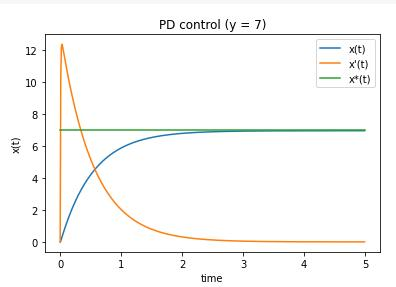
\includegraphics[width=1\linewidth]{images/output/300_150_0-C7.jpg}
            \caption{[PD] Not-tuned}
        \end{subfigure}
        \begin{subfigure}{.5\textwidth}
          \centering
          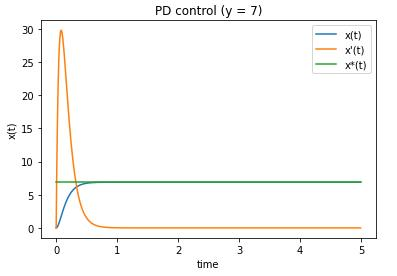
\includegraphics[width=1\linewidth]{images/output/143_12_0-C7.jpg}
          \caption{[PD] Tuned}
        \end{subfigure}
    \caption{Constant trajectory $x^*(t) = 7$}
    \label{fig:PD_const}
    \end{figure}
    
    \begin{figure}[htb]
        \begin{subfigure}{.5\textwidth}
            \centering
            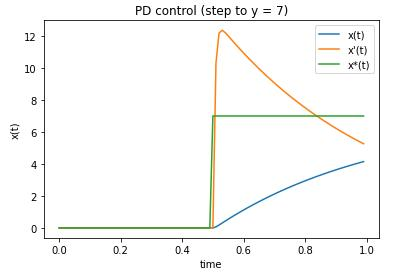
\includegraphics[width=1\linewidth]{images/output/300_150_0-S7.jpg}
            \caption{[PD] Not-tuned}
        \end{subfigure}
        \begin{subfigure}{.5\textwidth}
          \centering
          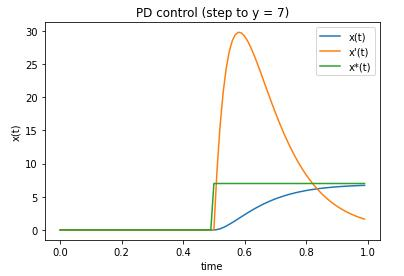
\includegraphics[width=1\linewidth]{images/output/143_12_0-S7.jpg}
          \caption{[PD] Tuned}
        \end{subfigure}
    \caption{Step trajectory}
    \label{fig:PD_step}
    \end{figure}
    
    \begin{figure}[htb]
        \begin{subfigure}{.5\textwidth}
            \centering
            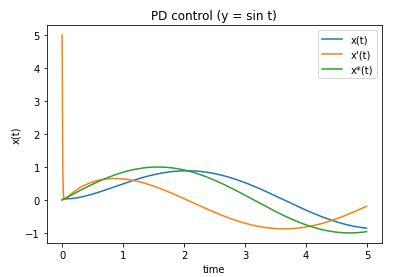
\includegraphics[width=1\linewidth]{images/output/300_150_0-sin.jpg}
            \caption{[PD] Not-tuned}
        \end{subfigure}
        \begin{subfigure}{.5\textwidth}
          \centering
          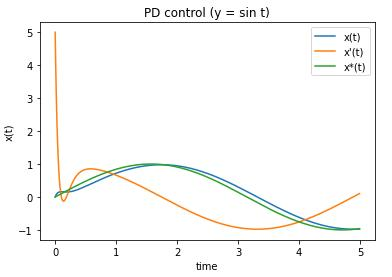
\includegraphics[width=1\linewidth]{images/output/143_12_0-sin.jpg}
          \caption{[PD] Tuned}
        \end{subfigure}
    \caption{Trajectory $x^*(t) = sin(t)$}
    \label{fig:PD_sin}
    \end{figure}
\newpage    
    \textbf{Result: } tuned controller converges faster.

\subsection*{Sub-task C}
    To prove that controlled dynamics is stable, lets consider the corresponding transfer function (\href{http://ctms.engin.umich.edu/CTMS/index.php?example=Introduction&section=ControlPID#16}{ref.}):
    \begin{equation*}
        \frac{K_d s + K_p}{s^2 + (\mu + K_d)s + (k + K_p)} = \frac{12 s + 143}{s^2 + 25s + 145} = \frac{12(s + 11.9167)}{(s + 9.1459)(s + 15.8541)}
    \end{equation*}
    Since all poles are negative the dynamics is stable.

\subsection*{Sub-task D}
    The question is how could we possibly implement a PD controller for system:
    \begin{equation*}
        \begin{bmatrix} 
            \dot x_1 \\ \dot x_2 \end{bmatrix} = 
        \begin{bmatrix} 
            10 & 3 \\
            5 & -5 
        \end{bmatrix} 
            \begin{bmatrix}x_1 \\ x_2 \end{bmatrix}
    \end{equation*}
    Implementing P controller is straight forward, problems arise with D component.\\
    For $2^{nd}$ and higher order systems we could calculate derivative error component as 
    \begin{equation*}
        current\_derivative = \frac{\Delta ERROR_P}{\Delta t}
    \end{equation*}
    Since we have an equation of first order, we will have the following situation:
    
    \begin{enumerate}
        \item Let $\begin{bmatrix}x_1 \\ x_2 \end{bmatrix} = X$ and 
        $
        \begin{bmatrix} 
            10 & 3 \\
            5 & -5 
        \end{bmatrix} = A$, thus we will have a system:
        
        \begin{equation*}
            \dot X = AX + Bu \text{ , where } u =K_d (\dot X -\dot  X^*) +K_p (X - X^*) 
        \end{equation*} 
    
        \item Substitution of $u$ will lead to:
        \begin{equation*}
            \dot X = AX - B K_d \dot X^* - B K_p X^* + B K_d \dot X + B K_p X
        \end{equation*}
        
        \begin{equation*}
            (I - B K_d ) \dot X = (A + B K_p) X - B(K_d \dot X^* + K_p X^*)
        \end{equation*}
        
        \item Let denote $ K_d \dot X^* + K_p X^* = C \equiv const$, so
        \begin{equation*}
            (I - B K_d ) \dot X = (A + B K_p) X - BC
        \end{equation*}
        
        \item There might also be a case that $\exists B^{-1}$ and $K_d = B^{-1}$, therefore:
        \begin{equation*}
            (A + B K_p) X = BC
        \end{equation*}
        
        \begin{equation*}
            X = (A + B K_p)^+ BC 
        \end{equation*}
        As a result, if $X \in col((A + B K_p)^+B)$, we have instantaneous change since we got rid of differentials, which is not physical. Similar should happen in general if we use a derivative of the same order as the equation in the control. So we shouldn't do this.
    \end{enumerate}

\newpage
\subsection*{Sub-task E}
    Figures \ref{fig:PI_PID_step} and \ref{fig:PI_PID_sin} compare PI and PID controllers on step and sine trajectories correspondingly.
    Coefficients for controllers:
    \begin{itemize}
        \item PI: $K_p = 36, K_i = 10$
        \item PID: $K_p = 36, K_d = 2, K_i = 9$
    \end{itemize}
    
    \begin{figure}[htb]
        \begin{subfigure}{.5\textwidth}
            \centering
            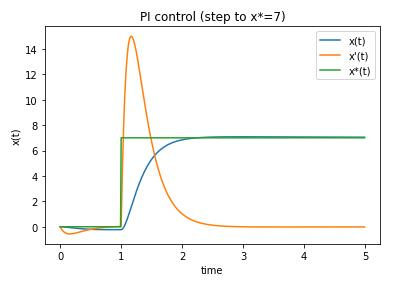
\includegraphics[width=1\linewidth]{images/output/36_0_10-S7.jpg}
            \caption{PI controller}
        \end{subfigure}
        \begin{subfigure}{.5\textwidth}
          \centering
          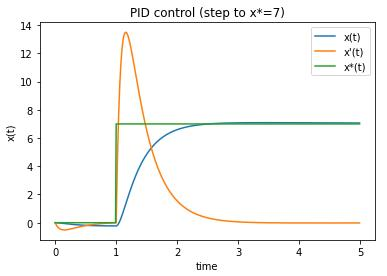
\includegraphics[width=1\linewidth]{images/output/36_2_9-S7.jpg}
          \caption{PID controller}
        \end{subfigure}
    \caption{Step trajectory}
    \label{fig:PI_PID_step}
    \end{figure}
    
    \begin{figure}[htb]
        \begin{subfigure}{.5\textwidth}
            \centering
            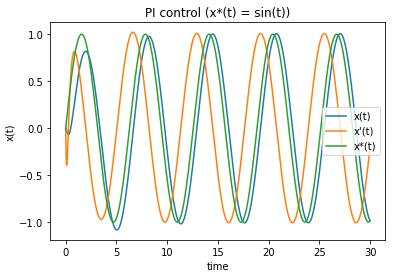
\includegraphics[width=1\linewidth]{images/output/36_0_10-sin.jpg}
            \caption{PI controller}
        \end{subfigure}
        \begin{subfigure}{.5\textwidth}
          \centering
          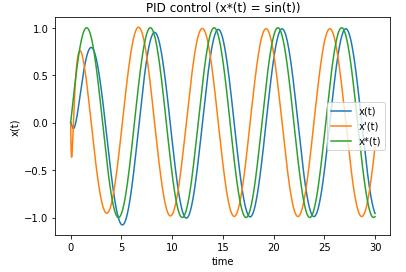
\includegraphics[width=1\linewidth]{images/output/36_2_9-sin.jpg}
          \caption{PID controller}
        \end{subfigure}
    \caption{Sine trajectory}
    \label{fig:PI_PID_sin}
    \end{figure}

\section*{Question 3}
\label{Q:3}
    The transfer function in my variant:
    \begin{equation*}
        W = \frac{s + 1}{s^3 +2s^2 + 9s + 20}
    \end{equation*}
    
    My actions were as follows:
    \begin{enumerate}[leftmargin=!,labelindent=5pt]
        \item Create a new model from "Feedback Controller" template. The schema is depicted on figure \ref{fig:schema}.
        \begin{figure}[H]
            \centering
            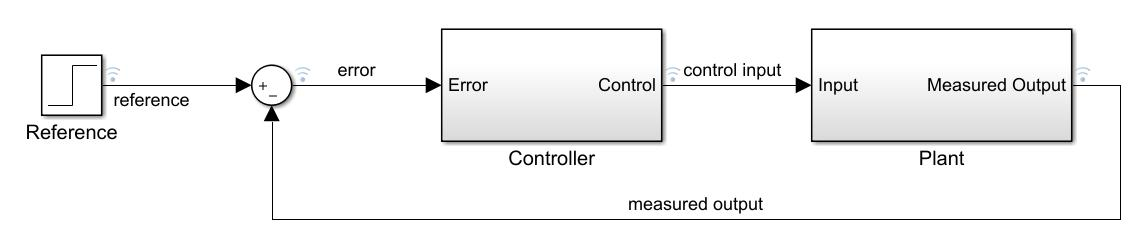
\includegraphics[width=15cm]{images/schemas/overall.jpg}
            \caption{Feedback controller}
            \label{fig:schema}
        \end{figure}
        
        \item Replace a plant for a given TF. The plant is shown on figure \ref{fig:plant}.
        \begin{figure}[H]
            \centering
            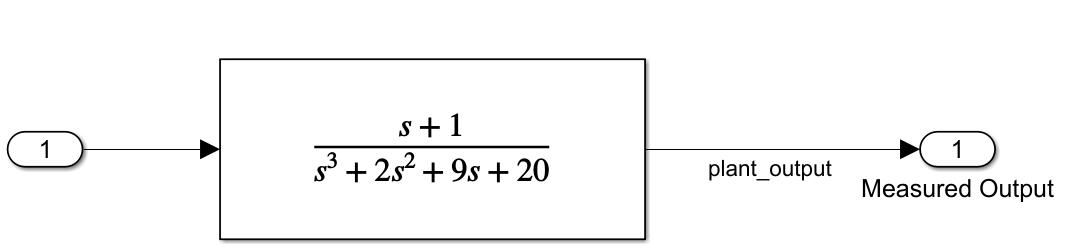
\includegraphics[width=15cm]{images/schemas/plant.jpg}
            \caption{The plant}
            \label{fig:plant}
        \end{figure}  
        
        \item Having inspected in-build "PID controller" block and understood that it provides noise filtering thus require additional coefficients, I decided to build the controller from scratch to keep simple classic model.
        
        \item Tune the controller using Matlab PIDtuner:
        \begin{enumerate}
            \item Open the tuner:
            \begin{verbatim}
>> transfer_func = tf([1 1], [1 2 9 20])

transfer_func =
 
          s + 1
  ----------------------
  s^3 + 2 s^2 + 9 s + 20
 
Continuous-time transfer function.

>> pidTuner(transfer_func, 'PID')
            \end{verbatim}
            
            \item In tuner play with response time and transient behavior to minimize overshoot. Figure \ref{fig:tuner} show the tuner's interface after tuning. Figure \ref{fig:tuned_params} shows tuned parameters. As we can see, there is still small overshoot of $0.0362\%$, but combining with small rise and settling time, the result is good. Final version of the controllers is at figure \ref{fig:controller}.
            \begin{figure}[H]
                \centering
                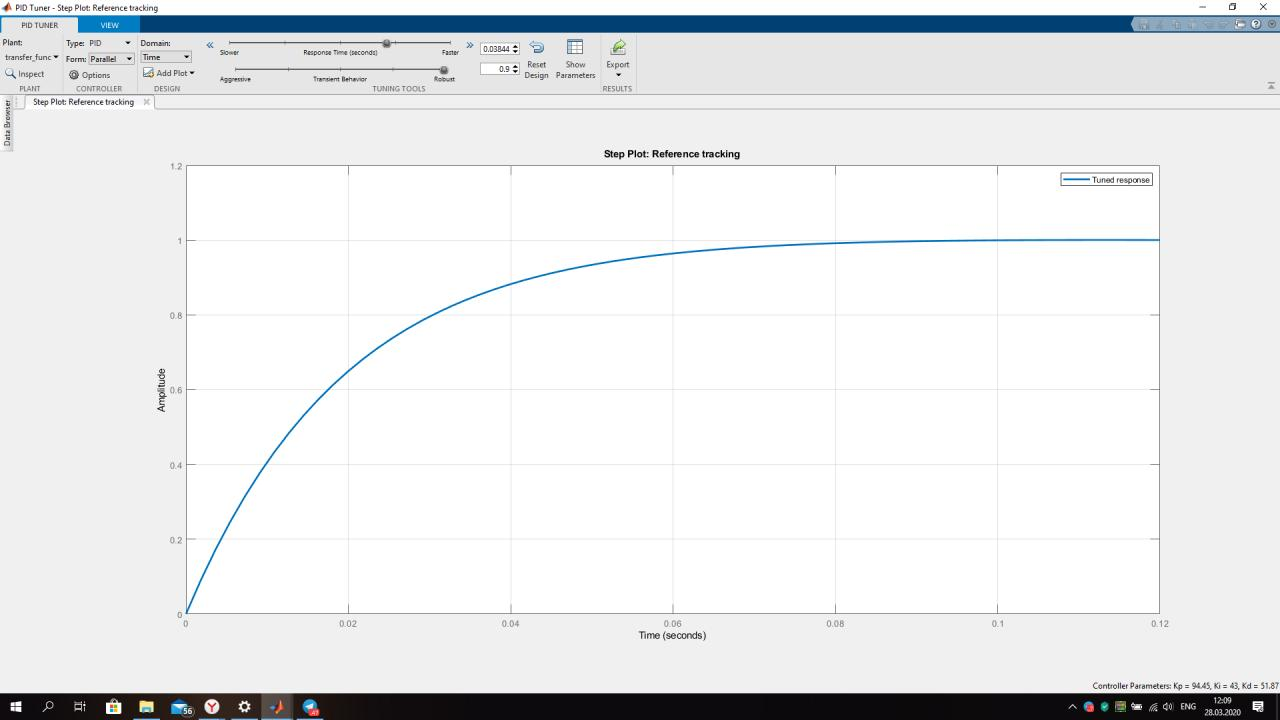
\includegraphics[width=15cm]{images/steps/tuner.jpg}
                \caption{Tuner}
                \label{fig:tuner}
            \end{figure} 
            
            \begin{figure}[H]
                \centering
                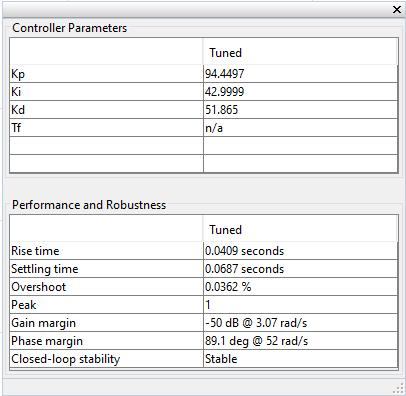
\includegraphics{images/steps/params.jpg}
                \caption{Parameters after the tuning}
                \label{fig:tuned_params}
            \end{figure} 
            
        \end{enumerate}
        
        \begin{figure}[H]
            \centering
            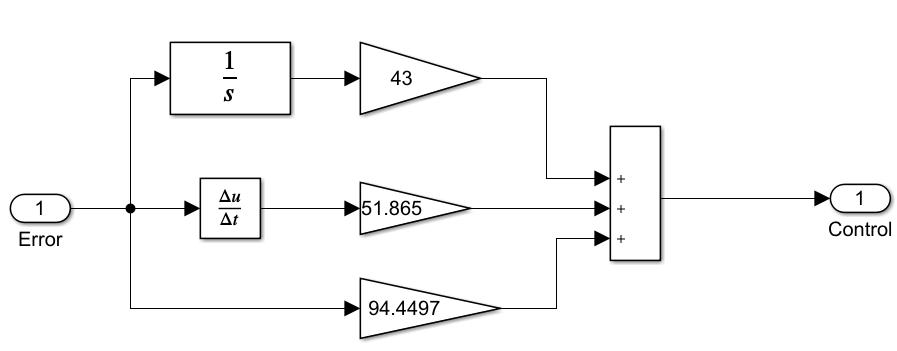
\includegraphics[width=15cm]{images/schemas/controller.jpg}
            \caption{The controller}
            \label{fig:controller}
        \end{figure}
        
        \item Build a schema to compare outputs with and without a controller. The result is at figure \ref{fig:comparison_schema}.
        \begin{figure}[H]
            \centering
            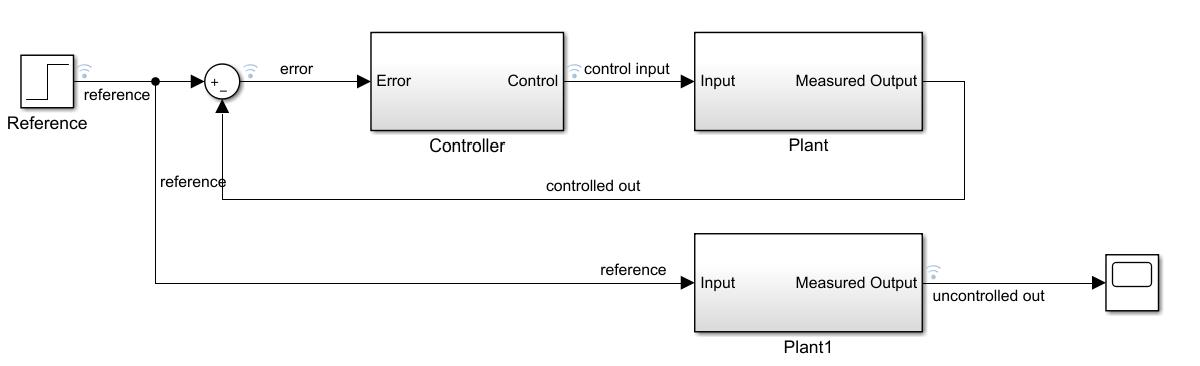
\includegraphics[width=15cm]{images/schemas/comparison_schema.jpg}
            \caption{The schema for comparison responses}
            \label{fig:comparison_schema}
        \end{figure}
        
        \item Mark signals to compare to be logged.
        
        \item Run simulation
        
        \item Inspect signals using data analyser. The comparison is shown at figure \ref{fig:comparison_out}. So we can see, that tuned PID controller really does its job well.
        \begin{figure}[H]
            \centering
            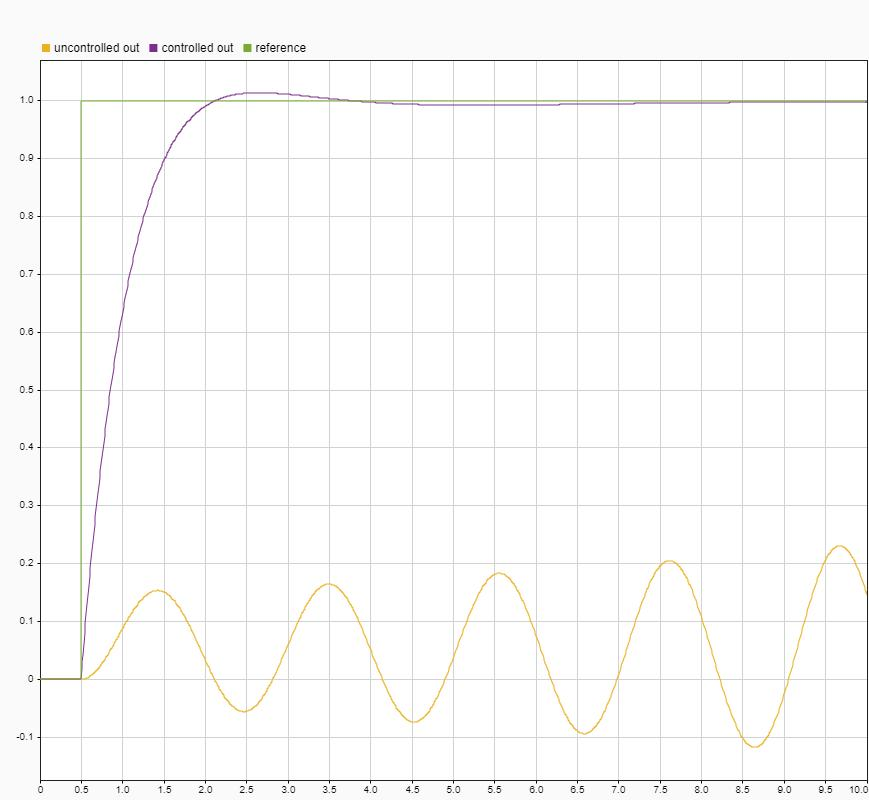
\includegraphics[width=15cm]{images/output/comparison_graphs.jpg}
            \caption{The signals' output}
            \label{fig:comparison_out}
        \end{figure}
    \end{enumerate}
    
\section*{Question 4}
\label{Q:4}
    The transfer function in my variant:
    \begin{equation*}
        W = \frac{s + 2}{s^2 + 4s + 11}
    \end{equation*}
    
    Figure \ref{fig:initial_metrics} shows Bode plot, Root Locus and Step Response of the initial system. As we can see, the system is stable, the only problem is that step response is to be tuned. An overshoot now is about $30\%$, increasing gain will lead to greater overshoot, therefore it is not a good idea.
    \begin{figure}[H]
        \centering
        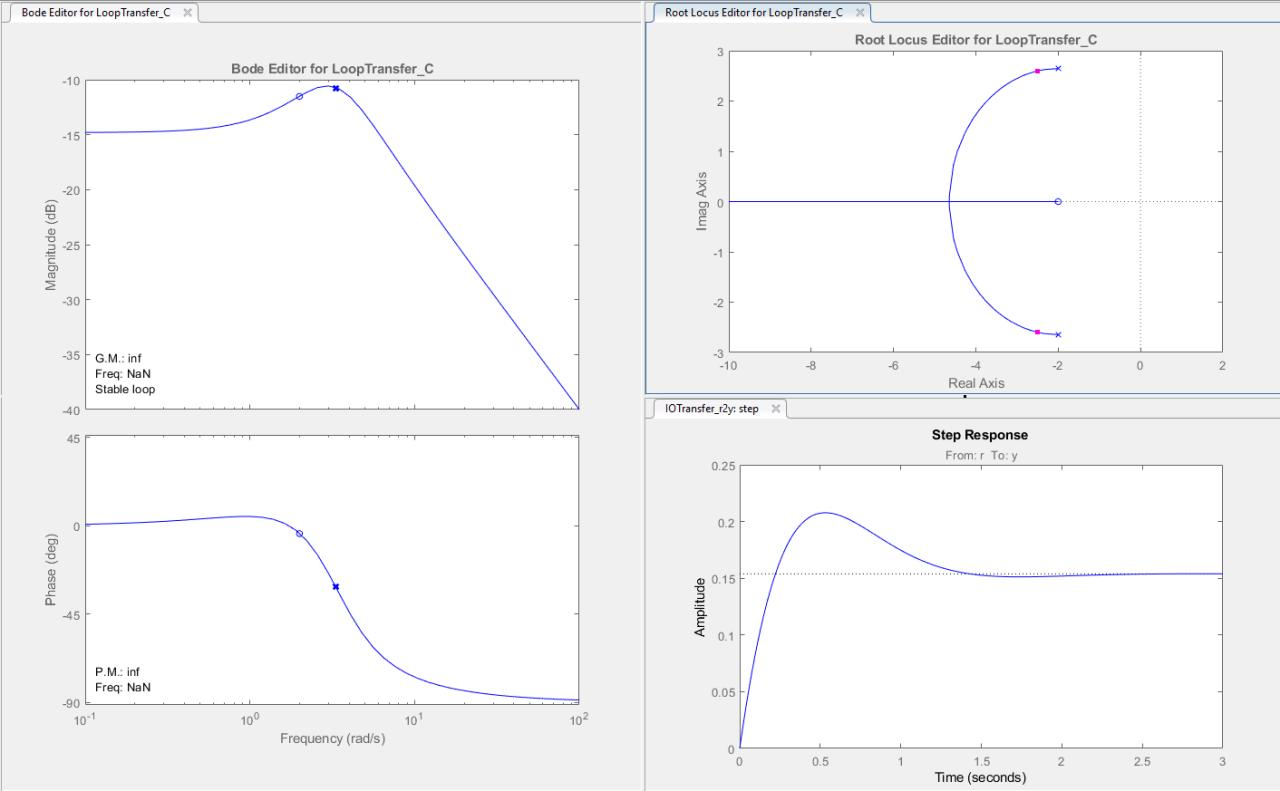
\includegraphics[width=16cm]{images/output/sys_init.jpg}
        \caption{Initial system metrics}
        \label{fig:initial_metrics}
    \end{figure}

    To make the situation better, let's introduce lead compensator via compensator editor:        
    \begin{equation*}
        5000\frac{s+1}{s+10}
    \end{equation*}
    
    So that the system metrics become much better (fig \ref{fig:tuned_metrics}):
    \begin{itemize}
        \item ~1\% steady-state error
        \item $1.5 \cdot 10 ^ {-3}$ sec rise and transient time
    \end{itemize}
    \begin{figure}[H]
        \centering
        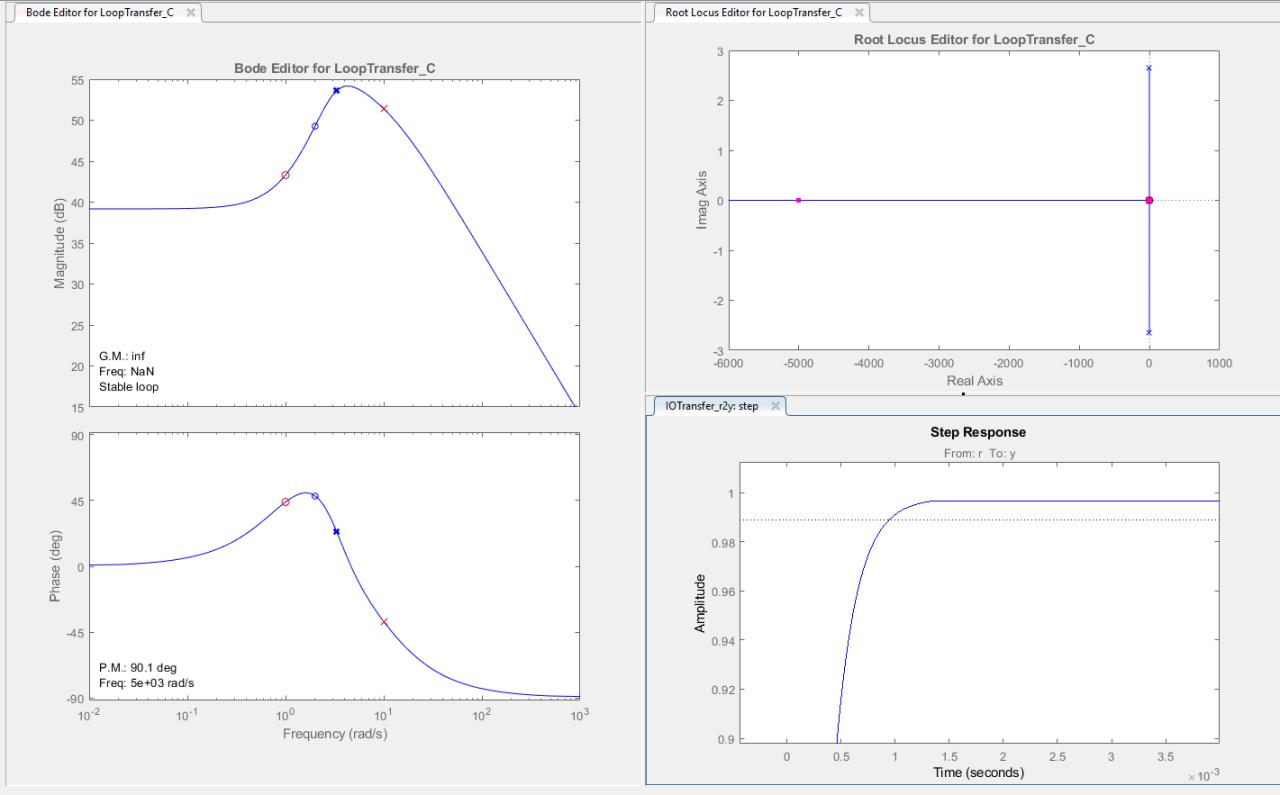
\includegraphics[width=16cm]{images/output/sys_tuned.jpg}
        \caption{Tuned system metrics}
        \label{fig:tuned_metrics}
    \end{figure}
    
    Increasing the coefficient to $10^5$ the system can have (fig \ref{fig:overtuned_metrics}):
        \begin{itemize}
        \item ~0.03\% steady-state error
        \item $10 ^ {-4}$ sec rise and transient time
    \end{itemize}
    \begin{figure}[H]
        \centering
        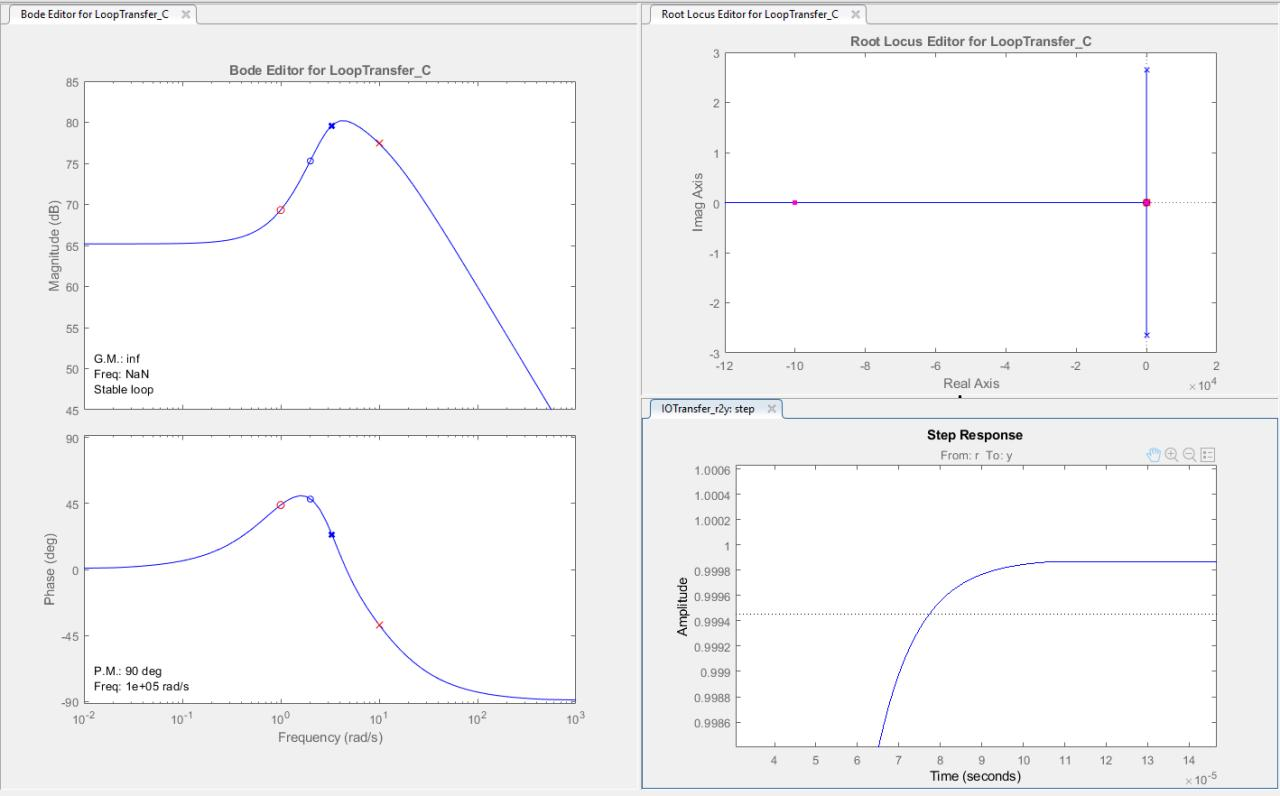
\includegraphics[width=16cm]{images/output/sys_overtuned.jpg}
        \caption{Over-tuned system metrics}
        \label{fig:overtuned_metrics}
    \end{figure}
    But usually nobody needs such precision, we 'over-tuned' the system.
\end{document}
